\documentclass[10pt,a4paper]{article}	
\usepackage{hyperref}
\usepackage{graphicx}
\usepackage{tabularx}
\usepackage[utf8]{inputenc}

\hypersetup{
colorlinks,
citecolor=black,
filecolor=black,
linkcolor=black,
urlcolor=black
}

\usepackage[a4paper,pdftex]{geometry}										% A4paper margins
\setlength{\oddsidemargin}{5mm}												% Remove 'twosided' indentation
\setlength{\evensidemargin}{5mm}

\usepackage[english]{babel}
\usepackage[protrusion=true,expansion=true]{microtype}	
\usepackage{amsmath,amsfonts,amsthm,amssymb}
\usepackage{graphicx}

\newcommand{\HRule}[1]{\rule{\linewidth}{#1}} 	% Horizontal rule

\makeatletter							% Title
\def\printtitle{%						
    {\centering \@title\par}}
\makeatother									
						

\title{\LARGE \textsc{Second Year Project} 	% Subtitle of the document
		 	\\[2.0cm]													% 2cm spacing
			\HRule{0.5pt} \\										% Upper rule
			\LARGE \textbf{\uppercase{Software Development in Large Teams with International Collaboration}}	% Title
			\HRule{2pt} \\ [0.5cm]								% Lower rule + 0.5cm spacing
			\normalsize \today		 % Todays date
			\\[3.0cm]							
		}





\begin{document}

\thispagestyle{empty}				% Remove page numbering on this page

\printtitle									% Print the title data as defined a		

{
\center 
Christian Martin Henriksen \texttt{cmah@itu.dk} \\ [0.5cm]
Helena Charlotte Lyn Kr\"uger \texttt{hclk@itu.dk} \\ [0.5cm]
Kasra Tahmasebi Shahrebabak \texttt{ktah@itu.dk} \\ [0.5cm]
Kewin Bent Pedersen \texttt{kbep@itu.dk} \\ [0.5cm]
Oliver Philip Roer \texttt{olpr@itu.dk} \\  [0.5cm]
Mathias Vildbrad \texttt{mhvi@itu.dk} \\[0.5cm] 
}

\newpage

\oddsidemargin 0.0in
\textwidth 6.5in

{\large Abstract} \\
Blabla bla we are awesome bla bla bla. \\
I suppose the singappl are ok too
\newpage

\tableofcontents

\newpage
\section{Introduction}
blablabla welcome
\section{Project ideas}
Project idea 
The idea for this project is called Common Knowledge. The idea is to make a service for schools, containing materials for each class’ curriculum. The institutions will pay to have an account, and can create accounts for its students and teachers.
We started out with brainstorming ideas for our project. Three ideas came up – Public Domain Library, Common Knowledge and IndieFlix, they are described below:\\\\
{\bfseries Public Domain Library}\\
After a certain amount of time, materials which are covered by copyright become public domain. The idea is to create a service that acts like a library, where people can upload and view content which has become public domain.\\\\
{\bfseries Common Knowledge}\\
As mobile entities like tablets and laptops are more and more used in schools, the students will with this idea be able to possess their curriculums electronically instead of on paper. This is a service containing all sorts of teaching media, only to be used by authorized teaching faculties, e.g. schools and universities. In order to satisfy copyright holders, a set fee might be charged in order to access the service.\\\\
{\bfseries Indieflix}\\
A service acting as a library of content from ‘indie’ producers of movies and series. The service would resemble YouTube to at some points, except only containing ‘indie’ content, fulfilling a certain quality standard.\\\\
When selecting one particular idea, we first eliminated Indieflix. We found it too monotonous as it would only regard videos. The choice was now between Common Knowledge and Public Domain Library.  We took three factors into consideration, they were; the features, the data model and the end user. As seen in the table below, Common Knowledge has more features and options to offer than Public Domain Library. More than that, it has specific end users, which are the schools and suppliers (for example Gyldendal). Public Domain Library has a more broad range of end users, and the challenges regarding the analysis of the end users and adapting the system are therefore limited. The data models for Public Domain Library and Common Knowledge are very different. We predict that the Public Domain Library will be a lot like the Singaporeans’ project idea, and therefore it will be more of a challenge to go with the Common Knowledge idea. This will force us to make an abstract data model, which will fit both SMU’s project and our own. We thought the PDL idea would be exciting, simple and fit our hobbies, but the above mentioned factors made us choose Common Knowledge as project idea.\\

\begin{tabularx}{\textwidth} {|X|X|}
\hline
\multicolumn{2}{|c|}{{\bfseries Feature Comparison}}\\
\hline
Public Domain Library & Common Knowledge \\
\hline
Content filtering & Access rights management \\
Streaming & Streaming\\
Banning of repeat offenders & Payments and cryptography\\
Accessible in browser & Distinct account types\\
Rating & Media rental\\
Calender for upcoming releases& Accessible in browser or through client software\\
Search and find structure & Material request system \\
& Catalog structure\\
& Search and find structure\\
\hline
\end{tabularx}

\section{Target-group analysis}
When analyzing the target group of our project idea, it is important to be aware of the fact that we do not approach the most active end user, who in our case is a student/teacher attending an institution. We need to keep our focus at the b2b-market, as the one purchasing the system is the institution and not the students/teachers. When looking at the b2b-market, we see that the buying decisions often is based on increasing profitability, reducing costs and enhancing productivity. Our system will focus on enhancing productivity. The requirements of the system will therefore mostly favour the institution rather than the students and teachers. 

Our group finds it important to be aware of who the target group is, as it is part of the foundation of our requirements. As an example we can look at the students/teachers as target group compared to the institution as target group. Our target group had a big influence on our choice of how to create a user. There were two options. We could let the students/teachers create a user themselves and have the institution accept them as belonging to that institution, or have the institutions create the users and hand them the password and username.
We agreed on having the institution as our target group, and chose to go with the second option. This would be easier for the institution, as we avoid spam and harassment from people not belonging to the institution and give our target group more control.

We can conclude that our target group is educational institutions, and we will, as stated above, define our requirements based on this.

\section{Specifications and use-cases}
\subsection{Service}
{\bfseries Tasks to be supported}\\
We decided among the group that the following are the tasks we want our webservice to support, based on our analysis of our target group:
\begin{itemize}
\item An user can log in.
\item An user of the system can upload various types of media, including, but not limited to:
\begin{itemize}
\item Text Documents
\item Pictures
\item Videos
\item Audio
\end{itemize}
\item An user can share access to and download a specified subset of the aforementioned  media.
\item A user can search through the content available to them.

\item An administrator can handle administration of user accounts.
\item A user can edit user rights to specific media if they are the owner or have editorial rights to it.
\end{itemize}

\begin{tabularx}{\textwidth} {|X|X|}
\hline
\multicolumn{2}{|c|}{T1: Creating users }\\
\multicolumn{2}{|l|}{Start: When a new student or teacher is included in the institution}\\
\multicolumn{2}{|l|}{End: The user is created with all information needed}\\
\multicolumn{2}{|l|}{Frequency: - }\\
\multicolumn{2}{|l|}{Difficult: When a new class starts}\\
\hline
Subtasks: & Example Solutions:\\
\hline
1. The admin/instituion logs in & System only shows the header, icon, login box and\\ 1a. The entered data does not match & perhaps info about the site, if 1a. shows an error message\\
\hline
2. Admin records user data & System requires mail, password and user type.
A\\
2a. User is already in the system  & confirmation message is shown - perhaps with info \\
2b. User is not in the system & about the user just created.\\
\hline
3. Admin gets and gives password to the user & Message is sent directly to the user. \\
\hline
\end{tabularx}
\\\\

{\bfseries Functional Requirements}\\
The following are the functional requirements we decided that our web service should meet:

\begin{itemize}
\item A user must be able to identify himself with the system, by having unique identifying accounts that a user can log into.
\item In order to log into his account, the user must provide a specific password.
\item The service must provide several different account types, having their own specific subset of the full privileges of the service.
\item A user must not be able to access any content if it is not logged in with an authorized account.
\item After a user has logged in, the service must maintain a login session, so that the user does not need authenticate itself again until he or she has logged out.
\item The service must be able to handle uploads of files in arbitrary formats.
\item A user must be able to access and download any media that they have rights to view.
\item An account that is capable of modifying access rights to certain content, must also itself, be able to access said content.
\item An account that is capable of accessing certain content, does not have to be able to modify access rights to said content.
\item Uploaded media must only be accessible to those accounts that own, or have obtained access to, that particular media.
\item Administrators have access to all media.
\item Administrators can manipulate access rights freely.
\item Accounts which upload content, must be able to manage access rights to said content.
\item Accounts capable of managing access rights to certain content, must be able to let other accounts manage rights to said content.
\item The service must provide means to which a user can look up and access the hosted content. These means will be in the form of:
\begin{itemize}
\item Search-and-find
\begin{itemize}
\item Users will type in what they are searching for. After confirming the search query, the service should display the best matches in the search results.
\end{itemize}
\item Catalogue
\begin{itemize}
\item A hierarchic structure in the form of links, in which users can look through available categories, choose a category, and then be lead to a list of content and/or sub-categories within the category.
\end{itemize}
\end{itemize}
\item Users must be able to attach metadata to the content they upload, including:
\begin{itemize}
\item Summary
\begin{itemize}
\item A short description of the content.
\end{itemize}
\end{itemize}
\begin{itemize}
\item Tags
\begin{itemize}
\item Keywords describing the content.
\end{itemize}
\end{itemize}
\item Creation of new users must be possible.
\item Users must be able to change their information.
\end{itemize}

{\bfseries Data Model}\\

\begin{figure}
\centering
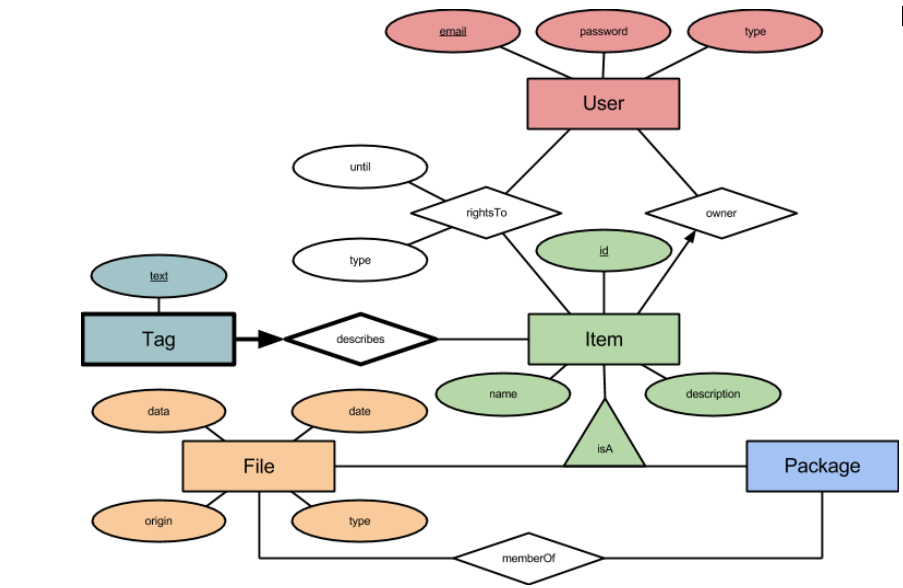
\includegraphics[width=14cm]{datamodel.png}
\caption{Our Data Model}
\label{dm}
\end{figure}
\newpage
\subsection{Client}
{\bfseries Requirements}\\
\begin{itemize}
\item The service must provide several different account types, having their own specific subset of the full privileges of the service. These account types include, but are not limited to:
\begin{itemize}
\item Student - The general “consumer” account.
\begin{itemize}
\item Will only be able to browse and download content.
\end{itemize}
\item Teacher - Part consumer, part content provider.
\begin{itemize}
\item Will be able to browse, download and upload content.
\end{itemize}
\item Institution - The customer.
\begin{itemize}
\item Will be able to create Student and Teacher accounts.
\item Will be able to distribute content to above accounts.
\end{itemize}
\item Supplier - The producer of the content.
\begin{itemize}
\item Will be able to upload and manage content.
\end{itemize}
\item Administrator
\begin{itemize}
\item Is able to create, read, update and delete all kinds of media and accounts.
\end{itemize}
\end{itemize}
\item Accounts cannot be made “from scratch” but must be created by other accounts.
\begin{itemize}
\item Administrator accounts will be available from the beginning.
\item Administrator accounts will be able to create accounts of all the different account types.
\item Supplier accounts cannot create new accounts.
\item Institution accounts can create Teacher/Student accounts.
\begin{itemize}
\item Institutions can then distribute its content to said accounts.
\end{itemize}
\end{itemize}
\item In order to access content, institutions must reach an agreement with a supplier.
\end{itemize}

\section{Project Management}
"SKRIVES TIL SIDST"
\section{Collaboration with Singapore Management University}

{\bfseries Getting to know each other}\\
Prior to the collaboration with the SMU team we had a video conference in order to get to know each other a bit better since we would spend the following weeks working with each other. The conference started out a bit awkward. Luckily, we had prepared an agenda beforehand, which gave the meeting a goal to work for us to reach. Using this agenda, the meeting became more structured which allowed it to proceed smoothly. We believe the video conference was a great success because it gave us an understanding of who we were going to work with. Also it made the future communication much easier as we, during the videoconference, got to know each other a bit and agreed on our choice of communication platforms.\\
A funny thing to mention that we learned during the videoconference is the fact that the Singaporeans weren’t quite as we expected/feared. Despite what we had read regarding Singaporeans they were almost like us. They had some sense of humor and weren’t afraid to tell their opinions. \\\\
{\bfseries Communication – Pros and cons}\\
One of the most important aspects of a project, especially when working with people on the other side of the globe, is communication. As we were not able to meet physically we had to communicate through digital media. Below we have listed the three different tools we have used to communicate and the pros and cons of each them. \\\\
{\bfseries Tools}\\
Initially we agreed on using Skype to keep in touch. It is easy to setup and use, and had both audio and video chatting capabilities. But the Singaporeans were not used to it, and they were therefore hardly ever available through Skype. Instead, we ended up using Facebook for daily exchanges of questions and comments. About once a week, we did a group meet-up using Google+ video chat Hangouts, where everyone could see each other face to face, and discuss things like we were sitting in the same conference room.\\\\
{\bfseries Workflow}\\
After the first video session our group agreed on communicating mostly through video conferences. Together with the SMU team, we agreed to aim at having one video conference each week, usually on Tuesday or Thursday afternoons, since our team would usually be present on ITU, and it wouldn’t be too late in Singapore at those times.
During the video conference set up by ITU we arranged one of our own using Google+ instead. At this meeting we discussed how we would like to shape the system. We had in advance written the functional requirements and data model. They had several comments and questions, but we found a solution both parties could agree on. After the meeting we started the actual work. The first thing we made was an ER model which would show the overall concept to the SMU team. This would ensure that we were talking about the same thing. Showing them our ER model quickly showed we weren’t quite on the same page. They couldn’t agree on our ER model which made it possible for us to have a reasonable debate regarding the shape of the project.\\
Once we both agreed on the ER model we started working on the interface. A lot of confusion appeared in the beginning of the project, as the Singaporeans thought they were supposed to make a client equal to ours. Because of this, a lot of questions about the intentions about our client  were asked during our video conference, and forced us to take a step back to internally discuss how to handle the situation. Once we got it all sorted out we could start working. After the meeting, we discussed in our team, how to handle this misunderstanding. We decided to let the SMU team develop their slightly similar client, since it wouldn’t be a problem to either part, and probably result in more confusion. In the first two weeks the Singaporeans dealt with the more visual related aspects of their client while we were busy developing the interface. Once we started rolling out some of the methods, our meetings with our SMU team became more frequent, as issues and methods had to be discussed.\\
The Singaporeans were disciplined and they were always prepared for the meetings. We made the agendas for the meetings, to make sure we wouldn’t waste time figuring out what to talk about. They were serious throughout the whole project and always ready to discuss the problems we would, encounter. As their programming experience was limited compared to ours, most of the web service interface design was ours to decide. They would however tell us if they believed they were in need of something or if the changes made wouldn't satisfy their needs for their client.\\\\
{\bfseries Scheduling issues}\\
Initially the collaboration with the group from Singapore seemed to work very well, but as the work progressed and we got further into the project problems started to occur.\\
The biggest problem during the collaboration was that the Singaporeans weren’t good at making demands on us - that is setting deadlines during the project instead of in the end. More than that, we didn’t check, when their final deadline was. This resulted in us planning our development poorly and a lot of stress at the end. This forced us into discarding a lot of final changes to the web service as the SMU group would not be able to apply the changes to their client. \\\\
{\bfseries Final thoughts}\\
We found the collaboration with the Singaporeans very interesting, and think we learned a lot from the experience. We did however end up with some issues regarding time-scheduling at the end of the collaboration. This ended up hurting the quality of the web service, which means our own client has to cope for these flaws. 






\section{WebService}
\subsection{Service Development Reflection}
At the end of our collaboration, we were still working on many additions to the web service. Because of the deadline, we were forced to cut many of these additions out of the final web service, as the SMU team didn’t have the time to involve it in their client.\\
These additions included:
\begin{itemize}
\item Allowing users to authenticate themselves by logging into the service.
\item Restricting access to content on the server to only those who have the rights to access that particular content.
\item Better error handling.
\item Functionality to better ensure state correctness of items in the database.
\end{itemize}
Some of these additions were meant to satisfy a part of the requirements of the service. Since they were not included in the service, it leaves the service in a non-complete state, in regards to the proposed requirements.\\
We believe that the development of the web service was going in the right direction. Apart from the few missing key components of the web service, we feel that the current state of the service reflects the actual finished service in a satisfying manner. With better time management, or more time to finish the service, we could have not only completely satisfied the requirements of the web service, but also have a more stable and consistent implementation of the web service.

\subsection{Code Documentation}
{\bfseries Data model thoughts/revisions}\\
In our first datamodel draft (see xxxx), we had the following structure:\\
A User was identified by email, and used a password for authorization purposes. The name was used for displaying purposes, and the type was used to distinguish between different users and their inherent privileges, e.g., a standard user was only allowed to perform certain actions, while an admin had no restrictions at all. In order to host content on our service, we made the File entity. On top of containing the actual file, File had a variety of attributes which would describe the actual contents of the file. Origin, type, description and date thus described who made the original content, the type of the content, a summary of the content and when the content was first published, respectively. Id was used for uniquely identifying a single file, and name for displaying the file textually. Lastly, owner stated which user claimed ownership of the file. Ownership was meant to be granted to the user who uploaded the file, and was required to always be filled out. This way, we could make sure that there would always be at least one user (besides the admins) who would be able to manage the file. The Tag entity was meant to mimic tag systems that could be found many places on the internet. A File was supposed to have zero, one or multiple tags, describing the contents of the file in one word for each tag. Thus, one would be able to look up files by tags (e.g. "software"), and also be able to quickly find other files that are (at the very least) slightly related. At this point, only the owner and admins would have access to a file. In order to share a file, the owner would have to put it in a package, maybe along with other files, and then share that package by granting other users rights to that package. A Package would be uniquely identified by its id, and the name would be used to display it textually. The description would, like with files, describe the contents of the package. Granted rights would be stored in the rightsTo relation. This relation tied an account together with a package, and had a read/manage attribute which stated what kind of rights the user in question had to the given package. Read would only allow the user to view the contents of the package, while manage would allow the user to also edit it. Lastly, an optional expiration date could be filled out, in order to restrict how long the user in question would be allowed to read/manage the package.\\
During the implementation of this data model, we encountered some hurdles that in turn brought some new ideas to the table. These ideas brought us to our final improved  data model (see xxxx). First off, when writing classes for EF (the Entity Framework), we noticed that File and Package had some similarities, more specifically, they both had names, id's and descriptions. Also, we would actually have preferred to be able to both tag and share files and packages, instead of only tagging files and sharing packages. This lead to the introduction of the Item entity. Item would thus contain any data that could describe either a file or a package, namely the unique integer id's, the name, description, their tags and their owners. A File would then have an is-a relationship with Item, supplying it it further with data, date, origin and type information which have already been explained. A Package would also have an is-a relationship with Item. The Package would then be an item that could contain zero, one or multiple files. We also had some great discussions, whether a package should contain items, that is both files and packages. We decided to discard the idea, since it would introduce a new set of problems, which we wouldn't have time to deal with, for example a package would be able to contain itself or have other kinds of cyclic references. Also, it would be able to have multiple references leading to the same files. All of these aspects would have to be handled in a smart way, and we thus decided that such a feature wasn’t worth the trouble.\\
The actual implementation of the data model was done using the code first approach with EF. We discovered this approach when researching on how to utilize EF, and it turned out to be a very intuitive and powerful way to model our data. Instead of dragging and dropping elements in a visual editor, followed by praying that it generates the expected code, we could easily translate our entities into C\# classes, which then would be turned into tables by the framework. More than that, the framework provided some powerful features we could benefit  from, e.g. annotations to enforce proper formatting of emails and a framework specific use of the 'virtual' keyword that would allow lazy loading of data members at runtime.

\subsection{Class/Code Explanation}
The code behind the service is structured as follows:\\
The web service interface is written as a C\# interface, and inherit by a concrete C\# class. This allow us to state the operations provided by the service in one place, and then provide the actual implementation in another. Most interactions with the service will result in further interactions with the underlying database. The implementation class will thus, for the most part, make further calls to a database controller class. This class will then handle the actual interactions with the database and perform the necessary checks and exception handling.\\
Many of these calls will involve what we refer to as our ‘entity classes/objects’ and ‘data contract classes/objects’. Lastly, we have enums that are common to both of these sets of classes.

\subsection{Entity-Framework}
Because of some incompatibilities between WCF (Windows Communication Foundation) and the classes we wrote for use with EF (the Entity Framework), we have introduced two sets of classes.\\
The Data Contract classes are intended to be used when interacting with the service, while the  Entity classes will only be used during interaction between the service and the underlying database. In order to translate between e.g. an Entity user and a Data Contract user, we have introduced explicit conversion operators in our Entity classes, which then allow us to easily convert an entity class to its corresponding datacontract class, and vice versa. We have decided to put the conversion operators in the Entity classes, and not the Data Contract classes, in order to prevent exposing them to clients, since they won't have any use outside the service. \\
By using this structure, it allow us to utilize the features of EF in our Entity classes, without any compromises, and also reduce bandwidth usage by keeping our Data Contract classes more lightweight.

\subsection{Test Strategy}
Before coding our program, we made a strategy for testing the system. We decided to use Code Contracts and Pex - a tool to generate unit tests from contracts. As we made the server, we wrote contracts to each method. Unfortunately, when we wanted to test the code, we discovered that Pex was only available to Visual Studio 2010 and not 2012, which we were using.  We thought we could install Visual Studio 2010 and use it to run Pex on our code, but our program file wasn't compatible, since it was written in 2012, and could therefor not be opened. \\
Our server was instead tested by our Singaporean team. s
 
\newpage

\section{Client}
this will be about client etc
\subsection{Platform considerations}
After the SMU-ITU collaboration ended, we had to decide on what technology our client implementation would make use of. Our requirements for the client, our previous experience in development in different platforms, and the state of the web service were the most influential factors in our choice of platform for our client implementation.\\
We had a discussion about details of the client, and agreed on the service’ current state not being as complete as we wanted it to be. Some functionalities were missing, and we decided to make up for it in the client. This decision increased the amount of work to do in the client, and we therefore chose to limit our choice of platform to the ones we had previous experience with. If we had chosen a platform none of the group members had previous experience with, it would grant the benefit of learning a new one altogether, but we felt it was more important to ensure the quality of the client.\\
Another decision we had to make was between having a client as an application that ran locally on the users computer, or keeping it as a web application. A local client would require a download before use, and keeping it updated would be harder. If some users were running old versions, we would have to decide on legacy support as well. In relation to the requirements of the client, there were no significant advantages on having the client run locally on the user machine.\\
We decided to use ASP.NET for the client. Implementing the client as a web application seemed like a better fit for the typical use of the program. The choice was also based on the experience some of the members of the group had with ASP.NET. This previous experience would be very beneficial, because the time spent on learning how to develop for the platform would be reduced, and this extra time could instead be used to improve the overall quality of the client.

\subsection{Class/code Explanation}
Stuff about code
\subsection{Mockups}
pretty drawings goes here
\subsection{Test Strategy}
testing stuff
\section{Reflection}
alt sådan noget discussion shit
\subsection{What did we learn}
\subsection{Goals}
\subsection{conclusion on test results}
\section{Appendix}
\subsection{Test tables}
\subsection{Old data models}
\subsection{Interface specification}


\end{document}